%------------------------------------------------------------------------------
\chapter{Results}
\label{ch:results}

Images everywhere and proper analysis of what the user is seeing, what is failing and why.
Include default Maya fire effect, pictures of fire from the papers mentioned in the previous work section and a historical overview on the improvements in the shaders.
Could also add some graphs with rendering times per light sample, decreased step, and with and without shadows.

In order to provide a wider comparison that is not only limited to academic results, we will also confront our results with work from industry software.
FumeFX~\cite{FumeFX} is a popular tool for modelling volumetric effects, it has been used in several films and video games, e.g. Ghost Rider 2, Thor, Green Lantern, Warhammer Online and Tomb Raider: Underworld.
A frame from a fire scene in Ghost Rider 2 is shown in Figure~\ref{fig:fumefx}.
Since \Maya was used as the base platform for the development of our software, an interesting comparison should include \Mayash's fire effect.
A simple scene with plane, a sphere, a cylinder and a light was created, as shown in Figure~\ref{fig:maya_no_fire_mental_ray}.
The result of rendering the scene with \Mayash's software renderer is shown in Figure~\ref{fig:maya_fire}, note how the sphere and cylinder do not experience any change in their illumination with respect to the scene without the fire.
If \MentalRay is used to render the same scene, the image shown in Figure~\ref{fig:maya_fire_mental_ray} is generated.
Although the fire itself looks more realistic, the only alteration in neighbouring objects  is the appearance of erroneous shadows.
Placing on the flame examples provided by \Maya in our test scene produced the result shown in Figure~\ref{fig:result_maya_fire_example}.
More specifically, the 14th frame of the simulation in the file fire fluid examples ``Flame.ma" was used.
Note that a point light had to be placed in the centre of the flame, and the emitted colour had to be matched manually to the fire colour, to be able to produce the desired effect.

All the images generated with our shader use 256 light samples, the volumes have resolutions of $256 \times 256 \times 256$ voxels and a ray march step size of half a voxel size.
To give some perspective of the evolution of the software, an image from an early stage of the application is shown in Figure~\ref{fig:result_early_stage}.
At that point standard ray marching was used, a white point light source was placed in the centre of the cube, and the colour of the volume was set manually to orange.
The final colour of each pixel was computed using alpha blending with the densities along the direction of the ray.
The shadows form due to an attenuation factor being computed in the shadow rays.

For the next step, we assume that our flame is a black body radiator, as shown in Figure~\ref{fig:result_blackbody}.
In each step of the ray marching, the 256 lights scattered throughout the fire are sampled to compute the colour.
Since no fuel is burning, there is no absorption coefficient to be computed, so the alpha blending is still used.

If we model the fire with a real fuel, for example propane, the image shown in Figure~\ref{fig:result_propane_shadows} is generated.
At this point we are rendering with the simplified RTE Equation~\ref{eq:rte_simplified}.
Note how the appearance of the flame improves significantly with respect to the previous result.
If we omit the computation of the attenuation factor for the emitted light $L_e$, rendering times are reduced significantly.
The result is shown in Figure~\ref{fig:result_propane}, the error incurred with this simplification is not unreasonable, as shown in Figures~\ref{fig:result_diff_shadow} and~\ref{fig:result_diff_shadow_x5}, computed as the absolute of the difference between both images.

\begin{figure}[htbp!]
	\centering
	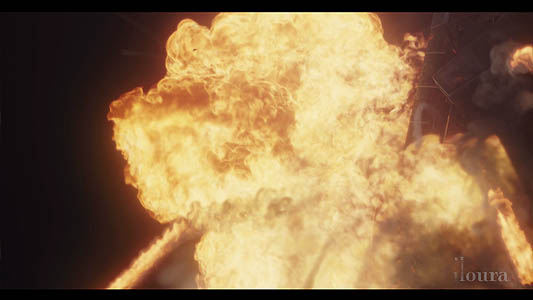
\includegraphics[width=\textwidth]{img/fumefx}
	\caption{Fire created with FumeFX~\cite{FumeFX}.}
	\label{fig:fumefx}
\end{figure}

\begin{figure}[htpb!]
        \centering
        \begin{subfigure}[t]{\textwidth}
                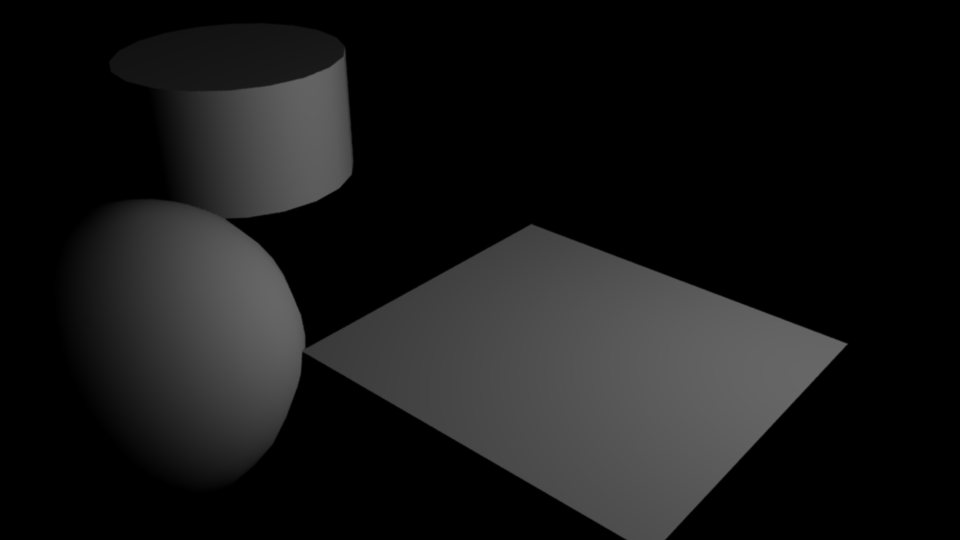
\includegraphics[width=\textwidth]{img/maya_no_fire_mental_ray}
                \caption{Scene without fire in \Maya, rendered with \MentalRay.}
                 \label{fig:maya_no_fire_mental_ray}
        \end{subfigure}    
        \\     
\end{figure}

\begin{figure}[htpb!]
		\ContinuedFloat
		\begin{subfigure}[t]{\textwidth}
                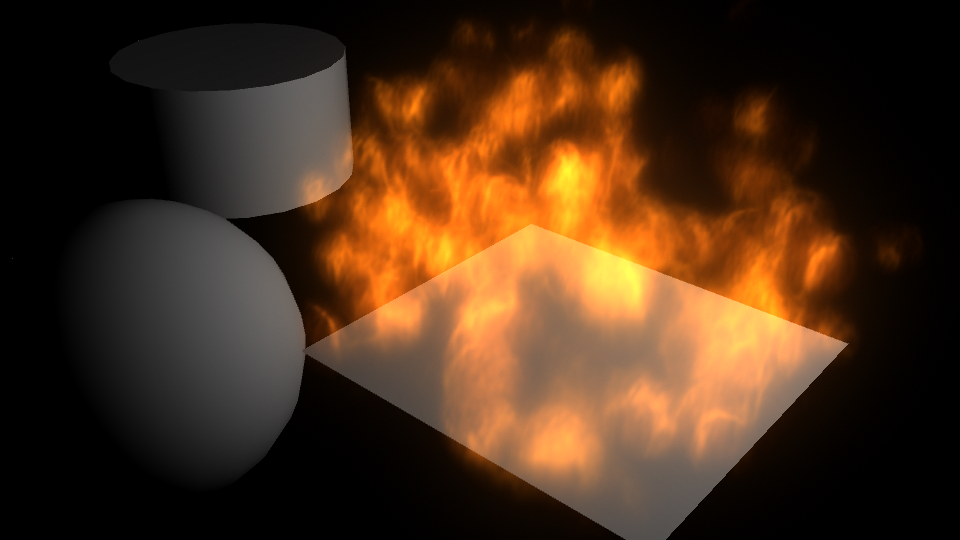
\includegraphics[width=\textwidth]{img/maya_fire}
                \caption{\Maya fire effect on a plane, rendered with \Maya software.}
                \label{fig:maya_fire}
        \end{subfigure}%        
\end{figure}

\begin{figure}[htpb!]
        \ContinuedFloat
 		\begin{subfigure}[t]{\textwidth}
                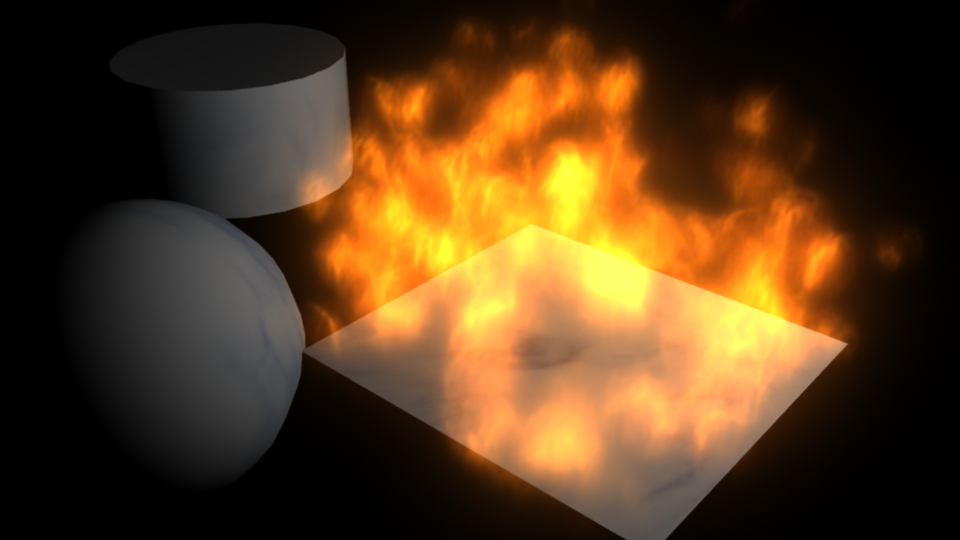
\includegraphics[width=\textwidth]{img/maya_fire_mental_ray}
                \caption{\Maya fire effect on a plane, rendered with \MentalRay.}
                \label{fig:maya_fire_mental_ray}
        \end{subfigure}%             
        \caption{Render tests for \Maya default fire effect.}
        \label{fig:maya_fire_scenes}
\end{figure}

\begin{figure}[htbp!]
	\centering
	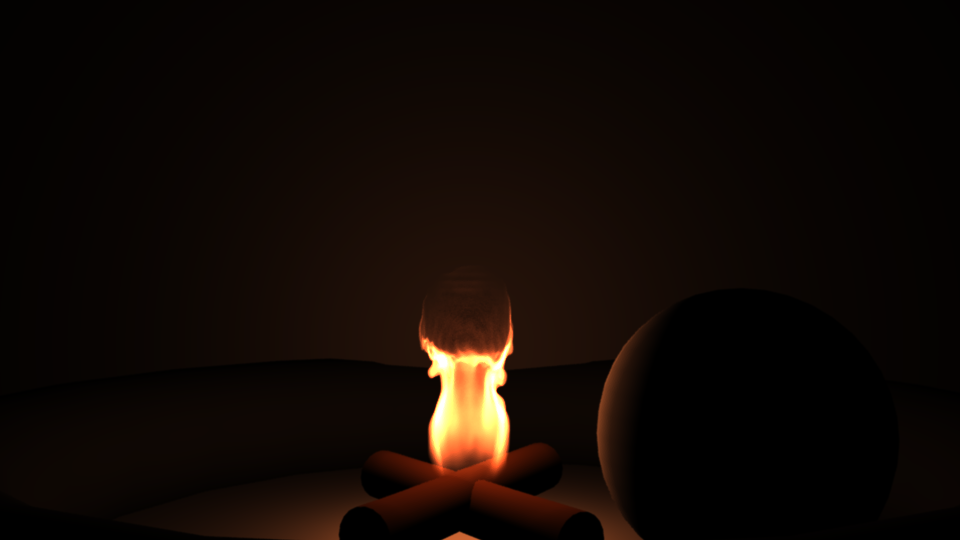
\includegraphics[width=0.8\textwidth, trim={8cm 0 8cm 10cm}, clip]{img/result_maya_fire_example}
	\caption{One of the \Maya fire fluid examples is our test scene.}
	\label{fig:result_maya_fire_example}
\end{figure}

\begin{figure}[htbp!]
	\centering
	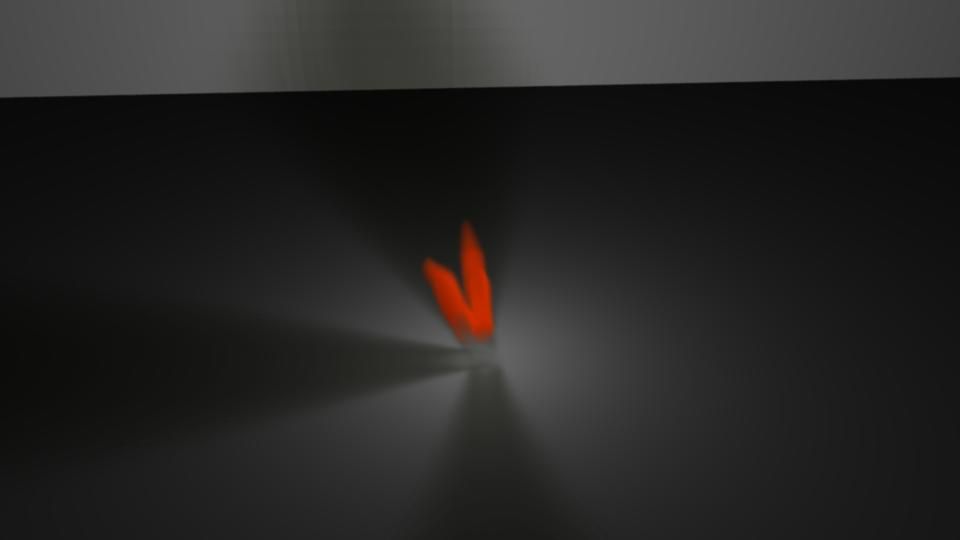
\includegraphics[width=\textwidth]{img/result_early_stage}
	\caption{Our renderer, early test, basic ray marching.}
	\label{fig:result_early_stage}
\end{figure}

\begin{figure}[htbp!]
	\centering
	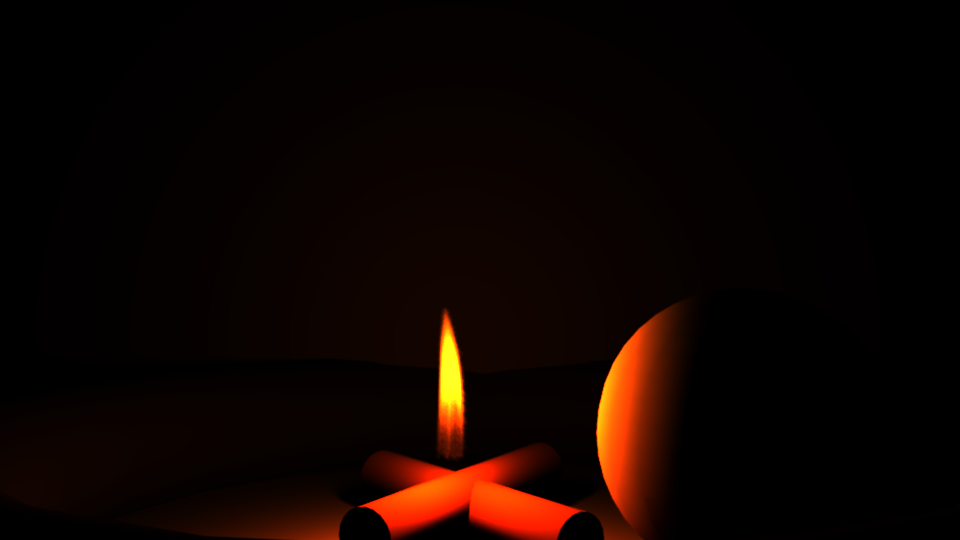
\includegraphics[width=0.8\textwidth, trim={8cm 0 8cm 10cm}, clip]{img/result_blackbody}
	\caption{result blackbody.}
	\label{fig:result_blackbody}
\end{figure}

\begin{figure}[htbp!]
	\centering
	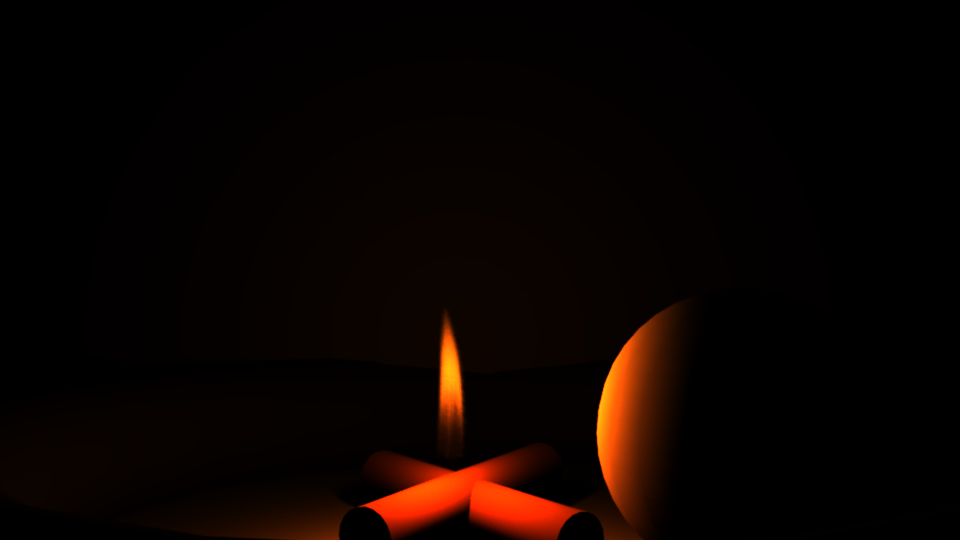
\includegraphics[width=0.8\textwidth, trim={8cm 0 8cm 10cm}, clip]{img/result_propane_shadows}
	\caption{Result propane full model.}
	\label{fig:result_propane_shadows}
\end{figure}

\begin{figure}[htbp!]
	\centering
	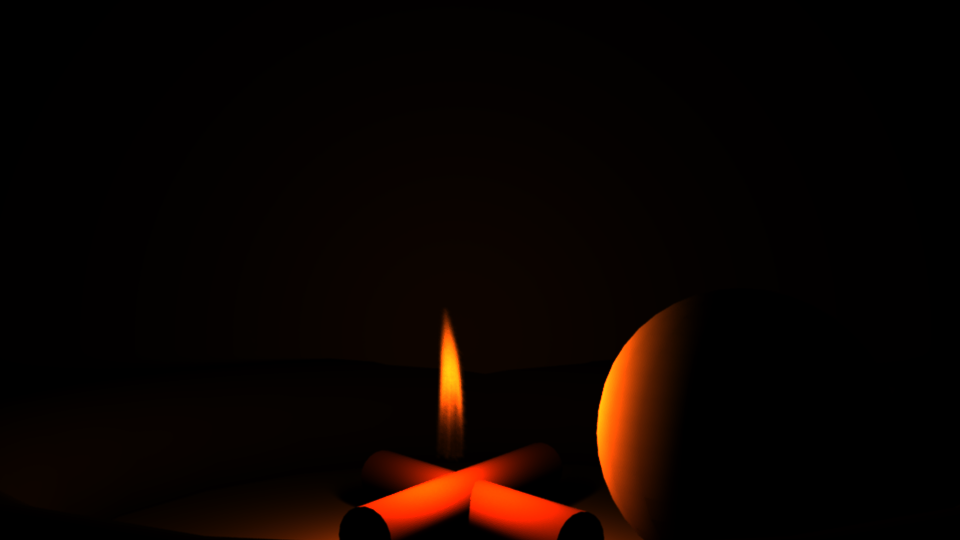
\includegraphics[width=0.8\textwidth, trim={8cm 0 8cm 10cm}, clip]{img/result_propane}
	\caption{result propane without shadows.}
	\label{fig:result_propane}
\end{figure}

\begin{figure}[htbp!]
	\centering
	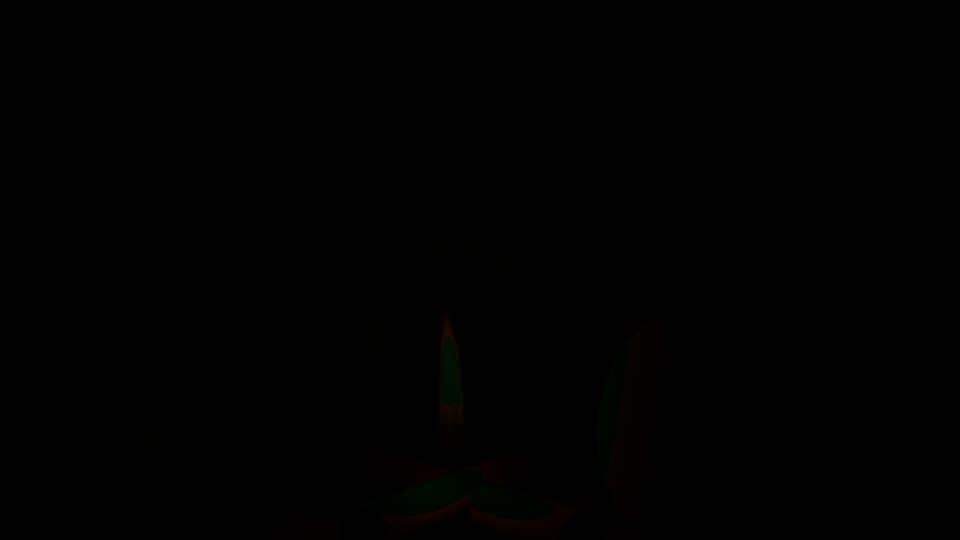
\includegraphics[width=0.8\textwidth, trim={8cm 0 8cm 10cm}, clip]{img/result_diff_shadow}
	\caption{Error introduced when the attenuation is not computed.}
	\label{fig:result_diff_shadow}
\end{figure}

\begin{figure}[htbp!]
	\centering
	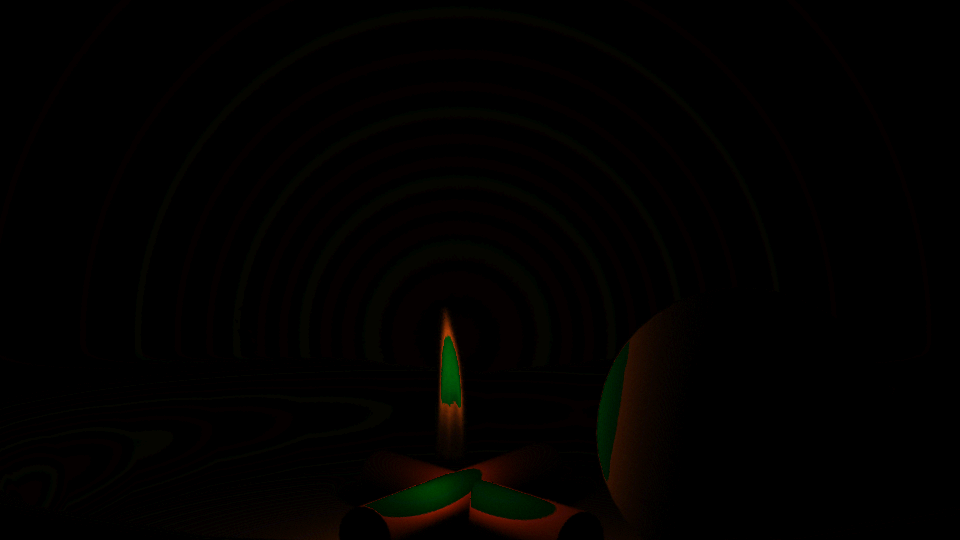
\includegraphics[width=0.8\textwidth, trim={8cm 0 8cm 10cm}, clip]{img/result_diff_shadow_x5}
	\caption{Previous error highlighted by a factor of 5.}
	\label{fig:result_diff_shadow_x5}
\end{figure}

\begin{figure}[htbp!]
	\centering
	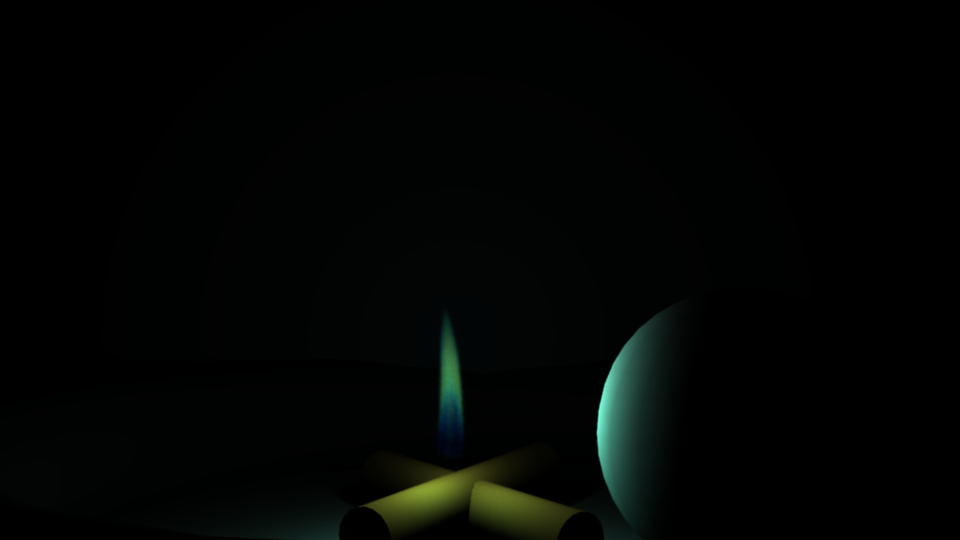
\includegraphics[width=0.8\textwidth, trim={8cm 0 8cm 10cm}, clip]{img/result_copper}
	\caption{result copper.}
	\label{fig:result_copper}
\end{figure}

\begin{figure}[htbp!]
	\centering
	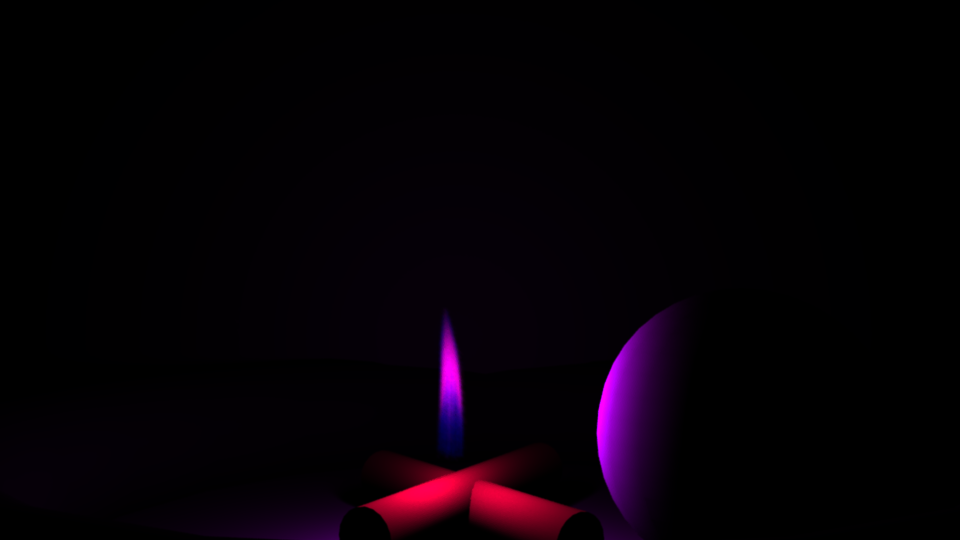
\includegraphics[width=0.8\textwidth, trim={8cm 0 8cm 10cm}, clip]{img/result_sulfur}
	\caption{result sulfur.}
	\label{fig:result_sulfur}
\end{figure}

\begin{figure}[htbp!]
	\centering
	
\includegraphics[width=0.25\textwidth]{img/result_synthetic}
	\caption{Our renderer, two flames superimposed.}
	\label{fig:result_synthetic}
\end{figure}